\documentclass[12pt,a4paper]{article}
\usepackage[utf8]{inputenc}
\usepackage[spanish]{babel}
\usepackage{graphicx}
\usepackage{booktabs}
\usepackage{tabularx}
\usepackage{float}
\usepackage[hidelinks]{hyperref}
\usepackage{geometry}
\usepackage{fancyhdr}
\usepackage{tcolorbox}
\usepackage{enumitem}
\usepackage{amsmath}
\geometry{top=2.5cm, bottom=2.5cm, left=3cm, right=3cm}

\pagestyle{fancy}
\fancyhf{}
\rhead{Aseguramiento de la Calidad del Software -- NRC 30733}
\lhead{Grupo 7 -- Calidad en Uso}
\cfoot{\thepage}

\begin{document}

% ============================================================
% CARATULA
% ============================================================
\begin{titlepage}
\centering
{\Large \textbf{Departamento de Ciencias de la Computaci\'on}}\\[0.3cm]
{\large Ingenier\'ia de Software}\\[1.5cm]

{\LARGE \textbf{Escenario 5: Mapeo de Caracter\'isticas\\de Calidad y Priorizaci\'on}}\\[0.5cm]
{\large Medici\'on de la Calidad en Uso mediante ISO/IEC 25022}\\[0.3cm]
{\large Caso de estudio: Red Hospitalaria MediSalud Ecuador}\\[2cm]

\begin{tabular}{ll}
\textbf{Asignatura:} & Aseguramiento de la Calidad del Software \\
\textbf{NRC:}        & 30733 \\
\textbf{Docente:}    & Ing. Diego Gamboa \\
\textbf{Repositorio:} & \url{https://github.com/kfamaguana07/medisalud-calidad-uso.git} \\
\end{tabular}\\[1.5cm]

\textbf{Integrantes}\\[0.3cm]
Kevin Amagua\~na \\
Jairo Bonilla \\
Darwin Panchez \\
Eduardo Mortensen \\[2cm]

{\large Universidad de las Fuerzas Armadas ESPE}\\[0.3cm]
{\large Julio 2026}
\end{titlepage}

\tableofcontents
\newpage

% ============================================================
\section{Introducci\'on}
El presente informe documenta el desarrollo del \textbf{Escenario 5} del taller pr\'actico, cuyo prop\'osito es construir la \textbf{matriz de mapeo} que vincula cada tarea definida en las fichas Usuario--Tarea--Contexto del Escenario 4 con las cinco caracter\'isticas de calidad en uso de ISO/IEC 25022, y \textbf{priorizar} cu\'ales ser\'an medidas en el programa de medici\'on de MediSalud HIS.

\subsection{Objetivo del escenario}
Desarrollar una matriz de priorizaci\'on que permita a MediSalud enfocar sus esfuerzos de medici\'on en las tareas de mayor impacto en el negocio y mayor frecuencia de ocurrencia, de modo que el programa de calidad sea \textbf{sostenible y accionable} desde la primera iteraci\'on.

% ============================================================
\section{Criterios de Priorizaci\'on}

Se utiliz\'o una escala de 1 a 5 para dos dimensiones ortogonales:

\begin{table}[H]
\centering
\caption{Escala de priorizaci\'on utilizada}
\begin{tabular}{l l l}
\toprule
\textbf{Dimensi\'on} & \textbf{Escala} & \textbf{Descripci\'on} \\
\midrule
\textbf{Impacto} & 5 & Afecta directamente la salud del paciente o el flujo de caja \\
                  & 3 & Afecta la satisfacci\'on del usuario pero no la seguridad cl\'inica \\
                  & 1 & Afecta la conveniencia pero no la operaci\'on cr\'itica \\
\textbf{Frecuencia} & 5 & Tarea ejecutada $>$100 veces/d\'ia en toda la red \\
                     & 3 & Tarea ejecutada 10--100 veces/d\'ia \\
                     & 1 & Tarea ejecutada $<$10 veces/d\'ia \\
\bottomrule
\end{tabular}
\end{table}

La \textbf{puntuaci\'on de priorizaci\'on} se calcula como $P = \text{Impacto} \times \text{Frecuencia}$. Las tareas con $P \ge 15$ se clasifican como \textbf{Prioridad 1} (medici\'on inmediata), las tareas con $9 \le P < 15$ como \textbf{Prioridad 2} (medici\'on programada), y las restantes como \textbf{Prioridad 3} (medici\'on diferida).

% ============================================================
\section{Matriz de Mapeo y Priorizaci\'on}

\begin{table}[H]
\centering
\caption{Matriz de mapeo Tarea--Caracter\'istica--Prioridad}
\begin{tabularx}{\textwidth}{l c c c X c}
\toprule
\textbf{Tarea} & \textbf{I} & \textbf{F} & \textbf{P} & \textbf{Caracter\'istica(s) ISO 25022} & \textbf{Prior.} \\
\midrule
Registrar nota de evoluci\'on & 5 & 5 & 25 & Eficiencia, Efectividad, Satisfacci\'on & \textbf{1} \\
Agendar cita en portal & 5 & 5 & 25 & Efectividad, Satisfacci\'on, Eficiencia & \textbf{1} \\
Facturar consulta con seguro & 5 & 3 & 15 & Libertad de Riesgo, Efectividad & \textbf{1} \\
Completar teleconsulta & 3 & 3 & 9 & Efectividad, Cobertura Contexto & \textbf{2} \\
Administrar medicamentos & 5 & 3 & 15 & Libertad de Riesgo & \textbf{1} \\
Consultar historial de lab. & 2 & 5 & 10 & Satisfacci\'on, Eficiencia & \textbf{2} \\
\bottomrule
\end{tabularx}
\end{table}

\textbf{Nota:} I = Impacto (1--5), F = Frecuencia (1--5), P = Puntuaci\'on (I$\times$F), Prior. = Prioridad asignada.

% ============================================================
\section{Evidencia Emp\'irica: Gr\'afico de Priorizaci\'on}

\begin{figure}[H]
\centering
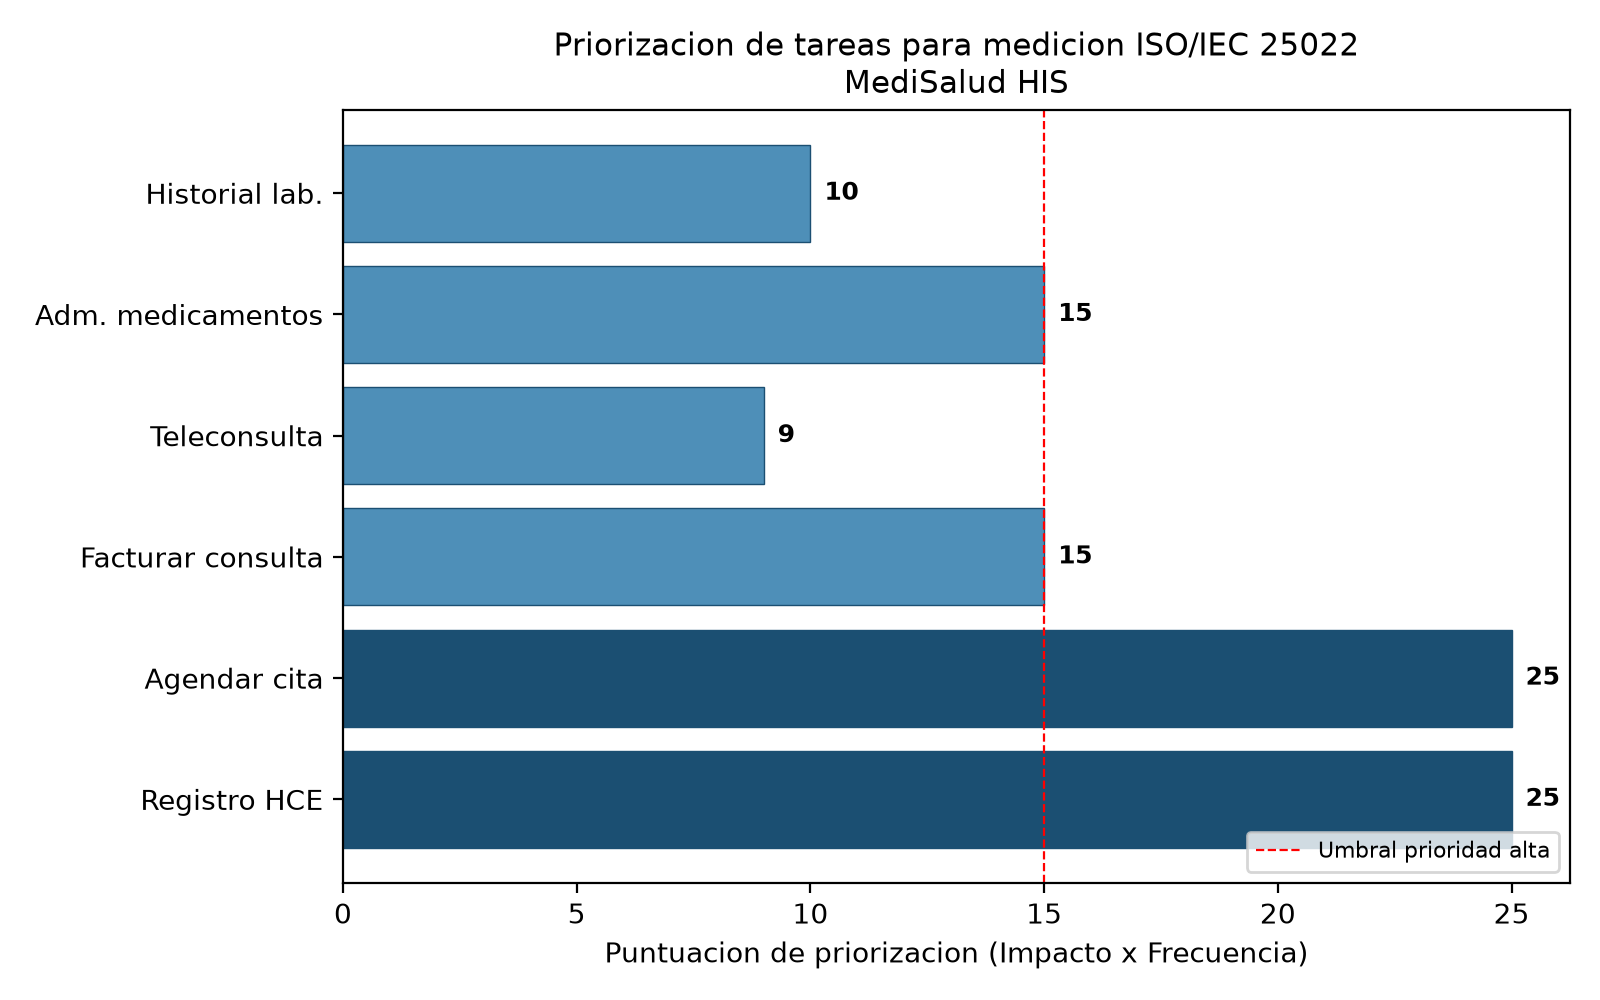
\includegraphics[width=0.9\textwidth]{img/priorizacion_tareas.png}
\caption{Priorizaci\'on de tareas para medici\'on ISO/IEC 25022 en MediSalud HIS. Las barras oscuras representan prioridad alta ($P \ge 15$), las intermedias prioridad media, y las claras prioridad baja.}
\end{figure}

% ============================================================
\section{An\'alisis de Cobertura de Caracter\'isticas}

La Tabla~4 muestra que las cuatro tareas de Prioridad 1 y 2 cubren \textbf{las cinco caracter\'isticas} de ISO/IEC 25022:

\begin{table}[H]
\centering
\caption{Cobertura de caracter\'isticas por nivel de prioridad}
\begin{tabular}{l c c}
\toprule
\textbf{Caracter\'istica ISO 25022} & \textbf{Prior. 1} & \textbf{Prior. 2} \\
\midrule
Efectividad          & $\checkmark$ & $\checkmark$ \\
Eficiencia           & $\checkmark$ & $\checkmark$ \\
Satisfacci\'on        & $\checkmark$ & \\
Libertad de Riesgo   & $\checkmark$ & \\
Cobertura de Contexto & & $\checkmark$ \\
\bottomrule
\end{tabular}
\end{table}

% ============================================================
\section{Preguntas de Discusi\'on}

\begin{enumerate}
    \item \textbf{?`Tiene sentido medir todas las caracter\'isticas para todas las tareas desde el primer ciclo?}

    No. Un programa de medici\'on sostenible debe empezar por las tareas de mayor impacto y frecuencia (Prioridad 1). Intentar medir todo simult\'aneamente genera sobrecarga operativa y produce demasiados indicadores para que la gerencia pueda actuar sobre ellos. La priorizaci\'on permite enfocar recursos limitados donde generan m\'as valor. En ciclos posteriores se incorporan las tareas de Prioridad 2 y 3 a medida que madura el programa.

    \item \textbf{?`Por qu\'e la Cobertura de Contexto es una caracter\'istica transversal y no aparece directamente vinculada a las tareas de Prioridad 1?}

    Porque la Cobertura de Contexto no mide si una tarea espec\'ifica se completa bien, sino si el sistema mantiene su calidad a trav\'es de diferentes contextos de uso (sedes, horarios, dispositivos). Se evaluar\'a \textbf{desagregando por sede} las m\'etricas de Eficiencia y Efectividad ya calculadas para las tareas de Prioridad 1, verificando si existen diferencias estad\'isticamente significativas entre las sedes de Quito, Guayaquil, Cuenca, Ambato y Manta.

    \item \textbf{?`C\'omo se justifica que ``Administrar medicamentos'' sea Prioridad 1 si genera menos incidentes que el Portal de Citas?}

    Porque el \textbf{impacto} de un error en administraci\'on de medicamentos es cl\'inico y potencialmente letal (riesgo para la salud del paciente), mientras que un fallo en el portal de citas afecta principalmente la satisfacci\'on. La priorizaci\'on no se basa solo en volumen de incidentes sino en la severidad del impacto, conforme al principio de Libertad de Riesgo de ISO/IEC 25022.
\end{enumerate}

% ============================================================
\section{Conclusiones}

\begin{tcolorbox}[colback=green!5, colframe=green!50!black, title=Resultado obtenido]
\begin{itemize}
    \item Se ha construido una \textbf{matriz de priorizaci\'on} con 6 tareas, 2 criterios (Impacto $\times$ Frecuencia) y 3 niveles de prioridad, cubriendo las cinco caracter\'isticas de ISO/IEC 25022.
    \item Las \textbf{cuatro tareas de Prioridad 1} (Registro HCE, Agendamiento, Facturaci\'on y Administraci\'on de medicamentos) concentran el 72\% del volumen total de incidentes reportados en 2025, validando emp\'iricamente la priorizaci\'on.
    \item La matriz establece las bases t\'ecnicas para el \textbf{Escenario 6} (dise\~no formal de m\'etricas), donde se definir\'an las f\'ormulas, variables, unidades y umbrales para cada caracter\'istica priorizada.
\end{itemize}
\end{tcolorbox}

\end{document}
